\chapter{Apéndices}
\label{ch:apendices}

%%%%%%%%%%%%%%%%%%%%%%%%%%%%%%%%%%%%%%%%%%%%%%%%%% GDD %%%%%%%%%%%%%%%%%%%%%%%%%%%%%%%%%%%%%%%%%%%%%%%%%%%%%%

\section{GDD (Documento de diseño de videojuegos)} \label{documento-diseño-videojuegos}

\subsection{Información general}

\subsubsection{Resumen del juego}
El juego consiste en una versión del juego cluedo que utiliza la Realidad Aumentada para renovar la forma de jugar a este juego, y a los juegos de mesa en general. El juego consiste en un tablero físico, sobre el que se mostrarán los elementos del juego de forma virtual con Realidad Aumentada. En él habrá habitaciones entre las que los personajes se tienen que mover para hacer deducciones y acusaciones, armas y personajes que servirán para dichas deducciones y acusaciones. Dichas acusaciones y deducciones contienen un posible asesino (personaje), una arma del asesinato y un lugar del asesinato.

\subsubsection{Objetivos a alcanzar por el juego}
Generar una versión de Cluedo con Realidad Aumentada que renueve la forma en que los juegos de mesa se relacionan con la tecnología, de forma que no sea el mismo juego en una pantalla, perdiendo toda la esencia de un juego de mesa. Si no que utilizando la Realidad Aumentada y las posibilidades que esta ofrece, generar una experiencia que iguale o incluso mejore a la original de los juegos de mesa, haciendo los juegos de mesa atractivos, tanto para los niños que se han criado con tecnología, por lo que la Realidad Aumentada llamará su atención, tanto como para los adultos que son fieles a los juegos de mesa tradicionales, que se sorprenderán por la increíble experiencia que aplicar la Realidad Aumentada a estos puede ofrecer.

\subsubsection{Justificación del juego}
Este juego supone una reinvención de los tradicionales juegos de mesa, una industria que debido a las nuevas tecnologías se queda atrás en términos de innovación. Esto puede cambiar con iniciativas como este juego que manteniendo la esencia de un juego de mesa, lo convierte en algo tecnológico e innovador, llamando así la atención de los amantes de los juegos de mesa, y a la vez de las nuevas generaciones, que no son usuarios asiduos de los juegos de mesa tradicionales.\\

Este juego es único gracias a su capacidad de a pesar de ser en su mayor parte virtual, al mismo tiempo mantener la sensación de ser un juego de mesa gracias al uso de la Realidad Aumentada, combina un factor tradicional con uno innovador, generando un nuevo concepto de los juegos de mesa que puede revolucionar el sector.\\

Por otro lado, este juego servirá para explorar las posibilidades que la realidad aumentada, y mas concretamente ARCore pueden ofrecer a los juegos de mesa tradicionales.

\subsubsection{Core gameplay}
El jugador tendrá que moverse por el tablero y intentar resolver el asesinato. Para moverse entre habitaciones tendrá que tirar el dado y en función del número podrá ir a una habitación o otra, el jugador puede hacer una acusación por turno en la que dice quien cree que cometió el asesinato y con que arma, la habitación de la deducción será en la que se encuentre el personaje actualmente. Entonces se le mostrará al jugador la interfaz para cambiar de turno en caso fallido, y la interfaz de finalización de juego en caso de acierto.\\

Al cambiar de habitación el jugador recibirá una pista sobre la nueva habitación, dichas pistas incluyen habitación, arma y personajes que no forman parte del asesinato, y siempre serán relacionados con esa habitación, por ejemplo, si se va a dar una pista, esta tendrá que ser sobre esa habitación o sobre las armas o personajes que estén dentro de esta.

El jugador dispone de una lista de elementos en los que puede ir marcando los que sabe que no forman parte del asesinato. Una vez el jugador crea que sabe el personaje, arma y habitación del asesinato puede hacer una acusación, si es acertada ganará.

\subsubsection{Características del juego}

\paragraph{Género}\mbox{}\\
El género de este juego es Estrategia, ya que tienes que llevar a tu personaje a las habitaciones adecuadas para resolver el crimen, en función de la nueva información que se va revelando cada turno de juego unas habitaciones serán más interesantes de visitar que otras y tienes que elaborar una buena estrategia para recorrer estas. También se hacen las deducciones de forma estratégica, para obtener antes la información del crimen, si por ejemplo, ya sabes que un arma y una habitación frman parte del crimen, puedes hacer una acusación con dicha arma, habitación y un personaje que quieras averiguar si forma parte del crimen o no.

\paragraph{Número de jugadores}\mbox{}\\
El juego esta diseñado para ser jugado por dos jugadores, y el objetivo de ambos es descubrir el asesinato antes que el otro, o en caso de que el otro haya fallado acertar el asesinato para ser él el ganador.

\paragraph{Plataforma de destino}\mbox{}\\
Este juego está destinado a móviles con sistema operativo Android que sean capaces de ejecutar ARCore.

\paragraph{Resumen de historia}\mbox{}\\
En una fiesta en la mansión de un adinerado señor en los años 80 ha habido un asesinato, y dicho señor ha sido la víctima. Uno de sus invitados ha sido el asesino y todos los invitados pasan la noche en la mansión hasta descubrir quién ha sido el asesino.

\subsubsection{Características del jugador}
\textbf{Perfil 1}: Hombres y mujeres de entre 25-45 años que se han criado con juegos de mesa y para los que dichos juegos son una parte importante de su entretenimiento. Estos usuarios encontrarán un juego de mesa renovado que utiliza la Realidad Aumentada, de forma que les ofrece una experiencia muy similar al juego de mesa tradicional que tanto les disfrutan pero con un toque totalmente renovado gracias al uso de esta nueva tecnología.\\

\textbf{Perfil 2}: Niños y niñas de entre 7-14 años que han crecido con las nuevas tecnologías y por tanto no suelen estar en contacto frecuentemente con juegos de mesa, pero que encontrarán en este una forma de jugar a algo tradicional, de una forma nueva y vistosa, que les llamará la atención gracias a los increíbles efectos visuales que aporta la Realidad Aumentada, introduciendo estos elementos virtuales en el mundo real.\\

\textbf{Perfil 3}: Jóvenes de entre 15-25 años, que han crecido con las nuevas tecnologías a la vez que los juegos de mesa tradicionales, por lo que están muy atados a ambos mundos y encontrarán en este juego la mezcla perfecta de ambos, utilizando el dispositivo móvil que están acostumbrados a usar a diario pero a la vez con un ambiente de juego de mesa tradicional al que tienen un apego por su infancia. Pertenecen además a una generación que ha crecido junto a los grandes avances de la tecnología en el siglo XXI, por lo que no son fáciles de convencer para decantarse por un juego determinado, pero a los que definitivamente fascinará la Realidad Aumentada y la nostalgia de un juego de mesa de su infancía.

\subsection{Mecánicas}
\subsubsection{Elementos del juego: Categorías}
\textbf{Arma}: Es un objeto que puede ser utilizado herir a un personaje. El objeto pertenece a la época de los años 80.\\
\textbf{Personaje}: Es un elemento que el jugador puede manejar o bien ser una parte más del juego. Hombre o mujer de entre 20-60 años perteneciente a los años 80. Ha ido a una fiesta en la mansión de un amigo, que ha sido asesinado durante dicha fiesta. Tiene la necesidad de descubrir quién ha sido el asesino. Puede ser el asesino.\\
\textbf{Habitación}: Es una estancia de una mansión. Pertenece a la época de los años 80.\\
\textbf{Útil}: Elemento del juego que ayuda al funcionamiento de éste.

\subsubsection{Elementos del juego: Núcleo principal}
\textbf{Srta. Amapola}: Pertenece a la categoría de elemento de juego “Personaje”. Tiene la capacidad de en caso de ser el personaje que el jugador ha elegido desplazarse entre las distintas habitaciones.\\
\textbf{Profesor Mora}: Pertenece a la categoría de elemento de juego “Personaje”. Tiene la capacidad de en caso de ser el personaje que el jugador ha elegido desplazarse entre las distintas habitaciones.\\
\textbf{Sra. Celeste}: Pertenece a la categoría de elemento de juego “Personaje”. Tiene la capacidad de en caso de ser el personaje que el jugador ha elegido desplazarse entre las distintas habitaciones.\\
\textbf{Coronel Rubio}: Pertenece a la categoría de elemento de juego “Personaje”. Tiene la capacidad de en caso de ser el personaje que el jugador ha elegido desplazarse entre las distintas habitaciones.\\
\textbf{Dra. Orquídea}: Pertenece a la categoría de elemento de juego “Personaje”. Tiene la capacidad de en caso de ser el personaje que el jugador ha elegido desplazarse entre las distintas habitaciones.\\
\textbf{Padre Prado}: Pertenece a la categoría de elemento de juego “Personaje”. Tiene la capacidad de en caso de ser el personaje que el jugador ha elegido desplazarse entre las distintas habitaciones.\\
\textbf{Cuerda}: Pertenece a la categoría de elemento de juego “Arma”. Estará en una habitación y cambiará a otra cuando en una deducción sea nombrada.\\
\textbf{Puñal}: Pertenece a la categoría de elemento de juego “Arma”. Estará en una habitación y cambiará a otra cuando en una deducción sea nombrada.\\
\textbf{Herramienta}: Pertenece a la categoría de elemento de juego “Arma”. Estará en una habitación y cambiará a otra cuando en una deducción sea nombrada.\\
\textbf{Pistola}: Pertenece a la categoría de elemento de juego “Arma”. Estará en una habitación y cambiará a otra cuando en una deducción sea nombrada.\\
\textbf{Candelabro}: Pertenece a la categoría de elemento de juego “Arma”. Estará en una habitación y cambiará a otra cuando en una deducción sea nombrada.\\
\textbf{Tubería de plomo}: Pertenece a la categoría de elemento de juego “Arma”. Estará en una habitación y cambiará a otra cuando en una deducción sea nombrada.\\
\textbf{Cocina}: Pertenece a la categoría de elemento de juego “Habitación”. Se encarga de albergar en su interior armas y personajes. Contiene un pasadizo secreto al Estudio por el que se puede desplazar un personaje sin tirar los dados.\\
\textbf{Comedor}: Pertenece a la categoría de elemento de juego “Habitación”. Se encarga de albergar en su interior armas y personajes.\\
\textbf{Salón}: Pertenece a la categoría de elemento de juego “Habitación”. Se encarga de albergar en su interior armas y personajes. Contiene un pasadizo secreto al Invernadero por el que se puede desplazar un personaje sin tirar los dados.\\
\textbf{Vestibulo}: Pertenece a la categoría de elemento de juego “Habitación”. Se encarga de albergar en su interior armas y personajes.\\
\textbf{Estudio}: Pertenece a la categoría de elemento de juego “Habitación”. Se encarga de albergar en su interior armas y personajes. Contiene un pasadizo secreto a la Cocina por el que se puede desplazar un personaje sin tirar los dados.\\
\textbf{Biblioteca}: Pertenece a la categoría de elemento de juego “Habitación”. Se encarga de albergar en su interior armas y personajes.\\
\textbf{Sala de billar}: Pertenece a la categoría de elemento de juego “Habitación”. Se encarga de albergar en su interior armas y personajes.\\
\textbf{Invernadero}: Pertenece a la categoría de elemento de juego “Habitación”. Se encarga de albergar en su interior armas y personajes. Contiene un pasadizo secreto al Salón por el que se puede desplazar un personaje sin tirar los dados.\\
\textbf{Sala de baile}: Pertenece a la categoría de elemento de juego “Habitación”. Se encarga de albergar en su interior armas y personajes.\\
\textbf{Dado}: Pertenece a la categoría de elemento de juego “Útil”. Se lanza al azar mostrando una de sus caras (que contiene un número de 1-6) como resultado de dicho lanzamiento.\\

\subsubsection{Reglas}
Si el jugador tira el dado, mostrar los posibles destinos en función de la habitación y el resultado del dado.\\

Si el jugador selecciona la habitación a la que desplazarse mover su personaje a dicha habitación.\\

Si el jugador hace acusación, comprobar que las cartas de la solución coinciden con las indicadas por el jugador, si asi es, mostrar un mensaje indicando que ha ganado, en otro caso mostrar la pantalla de cambio de turno, de forma que el realizar una acusación erronea implica el fin del turno del jugador actual.

\paragraph{Reglas de interacción}\mbox{}\\
La forma de interactuar es mediante botones, el jugador puede ir presionando los distintos botones que le permitirán tirar los dados, realizar acusaciones, moverse a otra habitación, etc.

\subsubsection{Elementos del juego: Mundo}
El mundo en este juego es tu propia realidad, al ser un juego de Realidad Aumentada, todo el mapa será tu habitación, pero no forma parte del juego, solo el tablero y sus alrededores.


\subsubsection{Elementos de registro y progreso}
Los elementos de registro son los jugadores, cada uno deberá elegir al personaje que quiere utilizar para jugar.\\

El progreso no se almacenará, una vez los jugadores abandonan una partida se tiene que volver a iniciar de nuevo.

\subsubsection{Elementos de jugabilidad y experiencia del jugador}
Todos los elementos 3D que serán situados en el mundo real gracias a la Realidad Aumentada permitirán una experiencia nueva para el jugador que rompe la barrera de lo real y lo virtual, permitiendo al jugador hacer todo desde su smartphone, pero haciendo que se sienta real, manteniendo así o mejorando la experiencia con los juegos de mesa.


\subsection{Dinámica}
\subsubsection{Mundo de juego. Universo virtual}
Al hacer uso de la realidad aumentada, el universo virtual será el mundo real, la habitación en la que estés, en dicho mundo se encontrará el tablero de juego sobre el que aparecerán los elementos 3D virtuales que permitirán al usuario jugar.

\paragraph{Detalles del juego en temática}\mbox{}\\
La ambientación del juego tiene que incluir misterio. Dejando al usuario con una sensación de intriga todo el rato.\\

La música también debe tener ciertos toques clásicos que mantengan un ambiente sofisticado.

\paragraph{Detalles del juego en temática}\mbox{}\\
Un adinerado señor de los 80 ha celebrado una fiesta en su mansión, y ha invitado a 6 amigos. Uno de estos amigos le asesina, pero nadie sabe quién ha sido, por tanto, estos 6 amigos pasan la noche en la mansión hasta averiguar quién ha sido el asesino, qué arma ha utilizado y en qué habitación lo ha hecho.\\

El juego comienza en el momento en que el anfitrión es asesinado y los amigos comienzan su acertijo para conocer la información del asesinato.\\

Esta historia es lineal, en todas las partidas es de la misma manera.

\subsubsection{Interfaz del juego}
Pantallas:
\begin{itemize}
  \item \textbf{Inicial}: En esta pantalla los jugadores tienen que elegir los personajes.
  \item \textbf{Instrucciones}: En esta pantalla los jugadores obitenen la información acerca del funcionamiento el juego.
  \item \textbf{Central}: Esta es la pantalla de juego, en la que se muestra a partir del tablero escaneado los elementos de juego.
  \item \textbf{Fin de partida}: En esta pantalla se indica al jugador que es el ganador.
\end{itemize}

\subsubsection{Controles de la interfaz}
El control de la interfaz va a ser en todo momento táctil, con botones que pueden ser pulsados en la propia pantalla.

\subsubsection{Aprendizaje del juego}
Cada vez que un jugador juega una partida, éste va a incrementar sus capacidades de deducción y estrategia, de forma, que en cada partida el usuario elegirá mejor a qué habitaciones dirigirse según la información obtenida previamente, y por tanto, conseguirá llegar a la solución del asesinato más rápido.

\subsubsection{Jugabilidad intrínseca}
El objetivo queda muy definidio desde el comienzo del juego, el ganador será el jugador que primero resuelva el asesinato.

\subsubsection{Jugabilidad artística}
La música inspira intriga todo el rato para mantener el ambiente de misterio.\\

En el momento de ganar la música inspira euforia, generando un momento épico para el jugador.

\subsubsection{Jugabilidad intrapersonal}
El jugador se siente intrigado todo el tiempo, y con la necesidad de descubrir quien ha cometido el asesinato.

\subsubsection{Jugabilidad interpersonal}
Los jugadores sienten rivalidad y la presión de ser el primero que descubre el asesinato, y por tanto, de ganar la partida.

\subsubsection{Restricciones comerciales}
La clasificación del juego debe ser para personas de 6 a 99 años.

\subsection{Información del documento}
\subsubsection{Definición, acrónimos y abreviaturas}
AR: Realidad Aumentada.\\


%%%%%%%%%%%%%%%%%%%%%%%%%%%%%%%%%%%%%%%%%%%%%%%%%%TABLA PRODUCT BACKLOG%%%%%%%%%%%%%%%%%%%%%%%%%%%%%%%%%%%%%%%%%%%%%%%%%%%%%%
\section{Product Backlog} \label{apendice-product-backlog}

En la Tabla \ref{tabla-product-backlog} podemos encontrar el Product Backlog.

\begin{table}[h]
  \begin{center}
    \begin{tabular}{|p{1cm}|p{7.5cm}|p{1.9cm}|p{1.6cm}|p{1.6cm}|}

      \hline
        \rowcolor{Gray} \textbf{ID}
        & \textbf{Título}
        & \textbf{Estimación}
        & \textbf{Iteración}
        & \textbf{Entrega}\\

      \hline
      HU1
      & Seleccionar personajes
      & 2
      & 3
      & 2\\

      \hline
      HU2
      & Comenzar juego
      & 3
      & 3
      & 2\\

      \hline
      HU3
      & Salir de la pantalla de instrucciones
      & 4
      & 3
      & 2\\

      \hline
      HU4
      & Escanear tablero
      & 5
      & 4
      & 2\\

      \hline
      HU5
      & Tirar los dados
      & 8
      & 5
      & 3\\

      \hline
      HU6
      & Seleccionar habitación a la que desplazarse
      & 2
      & 5
      & 3\\

      \hline
      HU7
      & Marcar carta con una X
      & 1
      & 6
      & 3\\

      \hline
      HU8
      & Desmarcar una carta
      & 2
      & 6
      & 3\\

      \hline
      HU9
      & Escanear una acusación
      & 8
      & 7
      & 3\\

      \hline
      HU10
      & Terminar partida
      & 2
      & 7
      & 3\\

      \hline
      HU11
      & Cambiar de turno
      & 1
      & 8
      & 4\\

      \hline

    \end{tabular}

    \caption{Listado del Product Backlog.}
    \label{tabla-product-backlog}

  \end{center}
\end{table}

%%%%%%%%%%%%%%%%%%%%%%%%%%%%%%%%%%%%%%%%%%%%%%%%TABLAS HISOTIRAS DE USUARIO %%%%%%%%%%%%%%%%%%%%%%%%%%%%%%%%%%%%%%%%%%%%%%%%%%%

\section{Historias de usuario} \label{historias-usuario}

\begin{table}[h]
  \begin{center}
    \begin{tabular}{|p{4cm}|p{4cm}|p{4cm}|}

    \hline
    \textbf{Identificador}: HU.1
    & \multicolumn{2}{p{8cm}|}{Seleccionar personajes}\\

    \hline
    \multicolumn{3}{|p{12cm}|}{\textbf{Descripción}: Como usuario jugador, quiero poder seleccionar un personaje de los disponibles en el juego.}\\

    \hline
    \textbf{Estimación}:2
    & \textbf{Prioridad}: 1
    & \textbf{Entrega}: 2\\

    \hline
    \multicolumn{3}{|p{12cm}|}{\textbf{Pruebas de aceptación}:
      \begin{itemize}
        \item Comprobar que los personajes elegidos se almacena correctamente.
      \end{itemize}
    }\\

    \hline

    \end{tabular}

    \caption{Tabla de la historia de usuario número 1.}
    \label{tabla-hu1}

  \end{center}
\end{table}

\begin{table}[h]
  \begin{center}
    \begin{tabular}{|p{4cm}|p{4cm}|p{4cm}|}

    \hline
    \textbf{Identificador}: HU.2
    & \multicolumn{2}{p{8cm}|}{Comenzar juego}\\

    \hline
    \multicolumn{3}{|p{12cm}|}{\textbf{Descripción}: Como usuario jugador, quiero poder comenzar el juego una vez seleccionados los personajes.}\\

    \hline
    \textbf{Estimación}:3
    & \textbf{Prioridad}: 1
    & \textbf{Entrega}: 2\\

    \hline
    \multicolumn{3}{|p{12cm}|}{\textbf{Pruebas de aceptación}:
      \begin{itemize}
        \item Comprobar que el juego avanza a la siguiente pantalla posterior a la inicial.
      \end{itemize}
    }\\

    \hline

    \end{tabular}

    \caption{Tabla de la historia de usuario número 2.}
    \label{tabla-hu2}

  \end{center}
\end{table}

\begin{table}[h]
  \begin{center}
    \begin{tabular}{|p{4cm}|p{4cm}|p{4cm}|}

    \hline
    \textbf{Identificador}: HU.3
    & \multicolumn{2}{p{8cm}|}{Salir de la pantalla de instrucciones}\\

    \hline
    \multicolumn{3}{|p{12cm}|}{\textbf{Descripción}: Como usuario jugador, quiero poder avanzar a la siguiente pantalla después de haber leído las instrucciones.}\\

    \hline
    \textbf{Estimación}:4
    & \textbf{Prioridad}: 1
    & \textbf{Entrega}: 2\\

    \hline
    \multicolumn{3}{|p{12cm}|}{\textbf{Pruebas de aceptación}:
      \begin{itemize}
        \item Comprobar que el juego avanza a la siguiente pantalla posterior a la de instrucciones.
      \end{itemize}
    }\\

    \hline

    \end{tabular}

    \caption{Tabla de la historia de usuario número 3.}
    \label{tabla-hu3}

  \end{center}
\end{table}

\begin{table}[h]
  \begin{center}
    \begin{tabular}{|p{4cm}|p{4cm}|p{4cm}|}

    \hline
    \textbf{Identificador}: HU.4
    & \multicolumn{2}{p{8cm}|}{Escanear tablero}\\

    \hline
    \multicolumn{3}{|p{12cm}|}{\textbf{Descripción}: Como usuario jugador, quiero escanear el tablero para que comience el juego.}\\

    \hline
    \textbf{Estimación}:5
    & \textbf{Prioridad}: 1
    & \textbf{Entrega}: 2\\

    \hline
    \multicolumn{3}{|p{12cm}|}{\textbf{Pruebas de aceptación}:
      \begin{itemize}
        \item Comprobar que se reconoce la imagen de tablero.
        \item Comprobar que se muestra la información 3D relacionada al tablero de forma correcta.
        \item Comprobar que se muestran los botones necesarios para el juego una vez escaneado el tablero.
      \end{itemize}
    }\\

    \hline

    \end{tabular}

    \caption{Tabla de la historia de usuario número 4.}
    \label{tabla-hu4}

  \end{center}
\end{table}

\begin{table}[h]
  \begin{center}
    \begin{tabular}{|p{4cm}|p{4cm}|p{4cm}|}

    \hline
    \textbf{Identificador}: HU.5
    & \multicolumn{2}{p{8cm}|}{Tirar los dados}\\

    \hline
    \multicolumn{3}{|p{12cm}|}{\textbf{Descripción}: Como usuario jugador, quiero tirar los dados para obtener el número de movimientos que tengo.}\\

    \hline
    \textbf{Estimación}:8
    & \textbf{Prioridad}: 1
    & \textbf{Entrega}: 3\\

    \hline
    \multicolumn{3}{|p{12cm}|}{\textbf{Pruebas de aceptación}:
      \begin{itemize}
        \item Comprobar que el lanzamiento de dados es aleatorio.
        \item Comprobar que se realiza correctamente el efecto visual.
        \item Comprobar que el jugador que ha tirado los dados puede desplazarse hasta donde la tirada de dados le permita.
      \end{itemize}
    }\\

    \hline

    \end{tabular}

    \caption{Tabla de la historia de usuario número 5.}
    \label{tabla-hu5}

  \end{center}
\end{table}

\begin{table}[h]
  \begin{center}
    \begin{tabular}{|p{4cm}|p{4cm}|p{4cm}|}

    \hline
    \textbf{Identificador}: HU.6
    & \multicolumn{2}{p{8cm}|}{Seleccionar habitación a la que desplazarse}\\

    \hline
    \multicolumn{3}{|p{12cm}|}{\textbf{Descripción}: Como usuario jugador, quiero poder seleccionar la habitación a la que desplazarme en función del número obtenido en el lanzamiento de dados.}\\

    \hline
    \textbf{Estimación}:2
    & \textbf{Prioridad}: 1
    & \textbf{Entrega}: 3\\

    \hline
    \multicolumn{3}{|p{12cm}|}{\textbf{Pruebas de aceptación}:
      \begin{itemize}
        \item Comprobar que el personaje se desplaza a la habitación seleccionada.
      \end{itemize}
    }\\

    \hline

    \end{tabular}

    \caption{Tabla de la historia de usuario número 6.}
    \label{tabla-hu6}

  \end{center}
\end{table}

\begin{table}[h]
  \begin{center}
    \begin{tabular}{|p{4cm}|p{4cm}|p{4cm}|}

    \hline
    \textbf{Identificador}: HU.7
    & \multicolumn{2}{p{8cm}|}{Marcar carta con una X}\\

    \hline
    \multicolumn{3}{|p{12cm}|}{\textbf{Descripción}: Como usuario jugador, quiero marcar una carta con una X.}\\

    \hline
    \textbf{Estimación}:8
    & \textbf{Prioridad}: 1
    & \textbf{Entrega}: 3\\

    \hline
    \multicolumn{3}{|p{12cm}|}{\textbf{Pruebas de aceptación}:
      \begin{itemize}
        \item Comprobar que se marca la carta indicada con una X.
      \end{itemize}
    }\\

    \hline

    \end{tabular}

    \caption{Tabla de la historia de usuario número 7.}
    \label{tabla-hu7}

  \end{center}
\end{table}

\begin{table}[h]
  \begin{center}
    \begin{tabular}{|p{4cm}|p{4cm}|p{4cm}|}

    \hline
    \textbf{Identificador}: HU.8
    & \multicolumn{2}{p{8cm}|}{Desmarcar una carta}\\

    \hline
    \multicolumn{3}{|p{12cm}|}{\textbf{Descripción}: Como usuario jugador, quiero desmarcar una carta.}\\

    \hline
    \textbf{Estimación}:2
    & \textbf{Prioridad}: 1
    & \textbf{Entrega}: 3\\

    \hline
    \multicolumn{3}{|p{12cm}|}{\textbf{Pruebas de aceptación}:
      \begin{itemize}
        \item Comprobar que se desmarca la carta.
      \end{itemize}
    }\\

    \hline

    \end{tabular}

    \caption{Tabla de la historia de usuario número 8.}
    \label{tabla-hu8}

  \end{center}
\end{table}

\begin{table}[h]
  \begin{center}
    \begin{tabular}{|p{4cm}|p{4cm}|p{4cm}|}

    \hline
    \textbf{Identificador}: HU.9
    & \multicolumn{2}{p{8cm}|}{Escanear una acusación}\\

    \hline
    \multicolumn{3}{|p{12cm}|}{\textbf{Descripción}: Como usuario jugador, quiero escanear las cartas para realizar una acusación.}\\

    \hline
    \textbf{Estimación}:8
    & \textbf{Prioridad}: 1
    & \textbf{Entrega}: 3\\

    \hline
    \multicolumn{3}{|p{12cm}|}{\textbf{Pruebas de aceptación}:
      \begin{itemize}
        \item Comprobar que se reconocen las cartas que forman parte de la acusación.
        \item Comprobar que la comprobación de si es la solución se hace de forma correcta.
        \item Comprobar que si la acusación es incorrecta pase al turno del siguiente jugador.
        \item Comprobar que si la acusación es correcta pase a la pantalla de victoria.
      \end{itemize}
    }\\

    \hline

    \end{tabular}

    \caption{Tabla de la historia de usuario número 9.}
    \label{tabla-hu9}

  \end{center}
\end{table}

\begin{table}[h]
  \begin{center}
    \begin{tabular}{|p{4cm}|p{4cm}|p{4cm}|}

    \hline
    \textbf{Identificador}: HU.10
    & \multicolumn{2}{p{8cm}|}{Terminar partida}\\

    \hline
    \multicolumn{3}{|p{12cm}|}{\textbf{Descripción}: Como usuario jugador, quiero terminar la partida.}\\

    \hline
    \textbf{Estimación}: 2
    & \textbf{Prioridad}: 1
    & \textbf{Entrega}: 3\\

    \hline
    \multicolumn{3}{|p{12cm}|}{\textbf{Pruebas de aceptación}:
      \begin{itemize}
        \item Comprobar que el juego cambia a la pantalla de inicio.
      \end{itemize}
    }\\

    \hline

    \end{tabular}

    \caption{Tabla de la historia de usuario número 10.}
    \label{tabla-hu10}

  \end{center}
\end{table}

\begin{table}[h]
  \begin{center}
    \begin{tabular}{|p{4cm}|p{4cm}|p{4cm}|}

    \hline
    \textbf{Identificador}: HU.11
    & \multicolumn{2}{p{8cm}|}{Cambiar de turno}\\

    \hline
    \multicolumn{3}{|p{12cm}|}{\textbf{Descripción}: Como usuario jugador, quiero cambiar de turno al del otro jugador.}\\

    \hline
    \textbf{Estimación}:1
    & \textbf{Prioridad}: 1
    & \textbf{Entrega}: 4\\

    \hline
    \multicolumn{3}{|p{12cm}|}{\textbf{Pruebas de aceptación}:
      \begin{itemize}
        \item Comprobar que el menú de anotaciones que se muestra a los jugadores es diferente.
        \item Comprobar que la información que se muestra sobre el tablero es diferente para los diferentes jugadores.
        \item Comprobar que efectivamente estamos en el turno del otro jugador (comprobando que la información que se muestra es la del otro jugador).
      \end{itemize}
    }\\

    \hline

    \end{tabular}

    \caption{Tabla de la historia de usuario número 11.}
    \label{tabla-hu11}

  \end{center}
\end{table}

\FloatBarrier

%%%%%%%%%%%%%%%%%%%%%%%%%%%%%%%%%%%%%%%%%%%%%%%%%%%%%% BOCETOS %%%%%%%%%%%%%%%%%%%%%%%%%%%%%%%%%%%%%%%%%%%%%%%%%%%%%%

\section{Bocetos} \label{bocetos}

Las siguientes imágenes recogen los bocetos realizados previos al desarrollo del juego.\\

\begin{figure}[h]
  \centering
  \subfigure{
  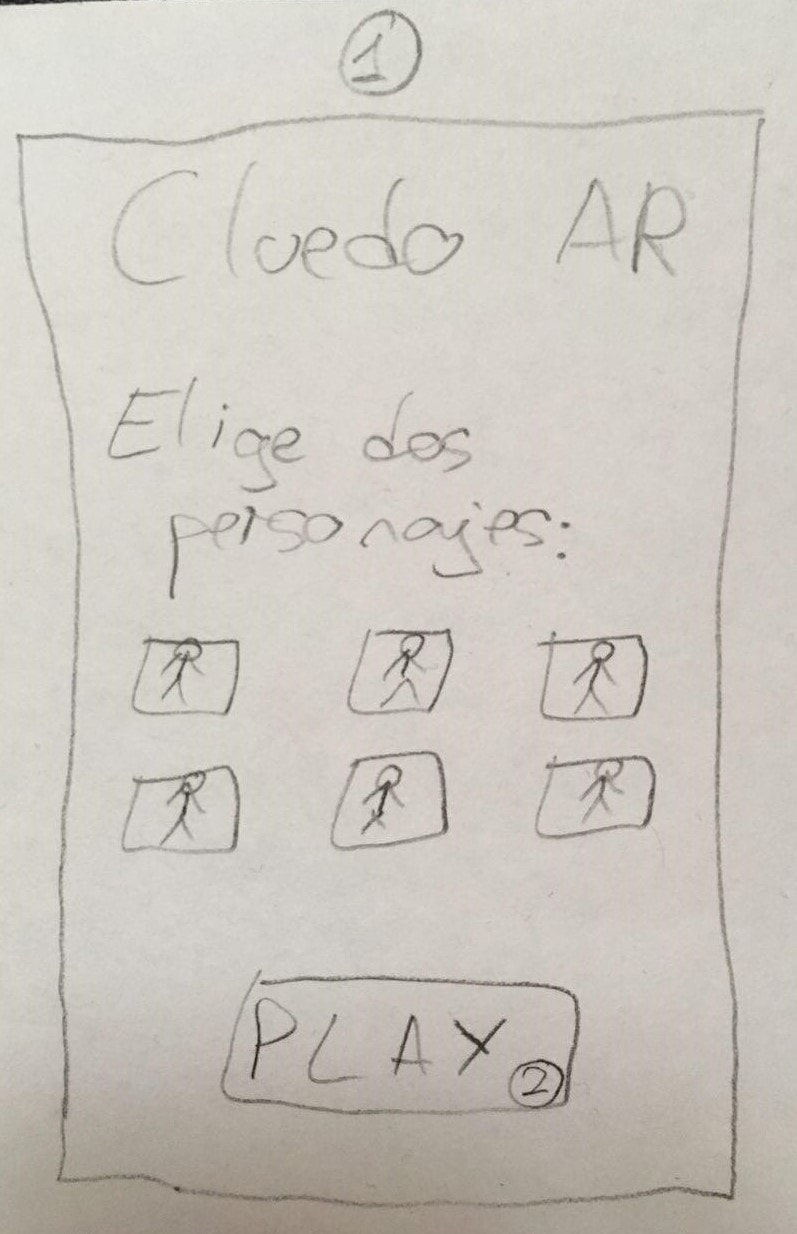
\includegraphics[height=2.48in]{b1.jpg}}
  \qquad
  \subfigure{
  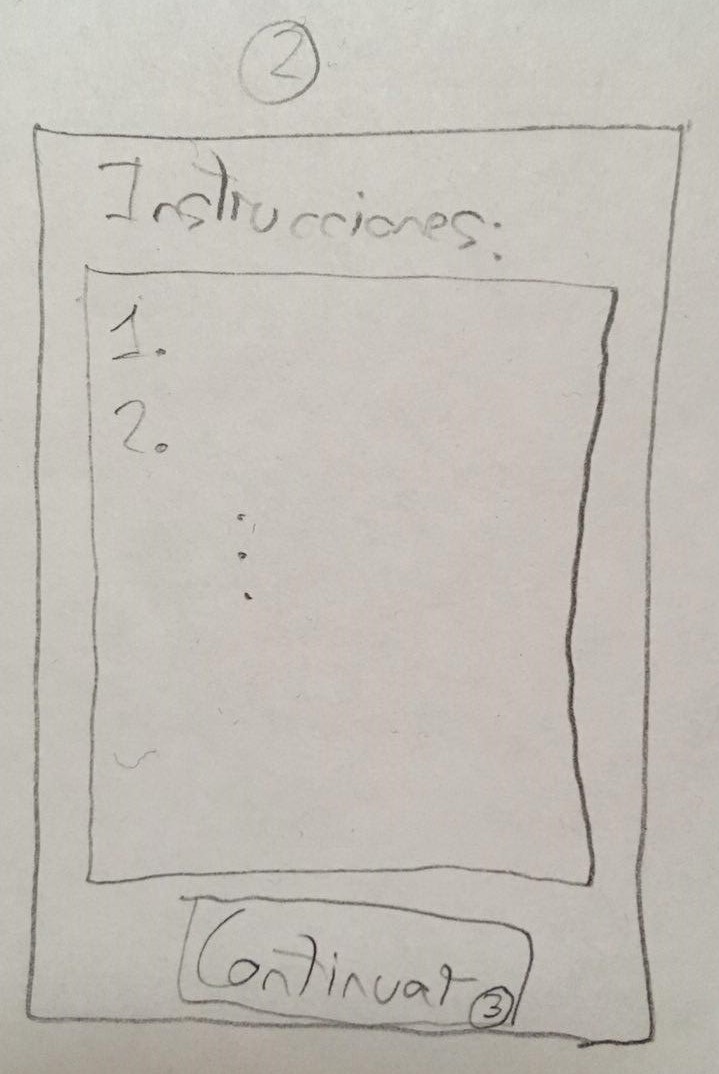
\includegraphics[height=2.48in]{b2.jpg}}
  \caption{Imagen que muestra los bocetos correspondientes a la interfaz inicial y la interfaz de instrucciones.}
\end{figure}

\begin{figure}[h]
  \subfigure{
  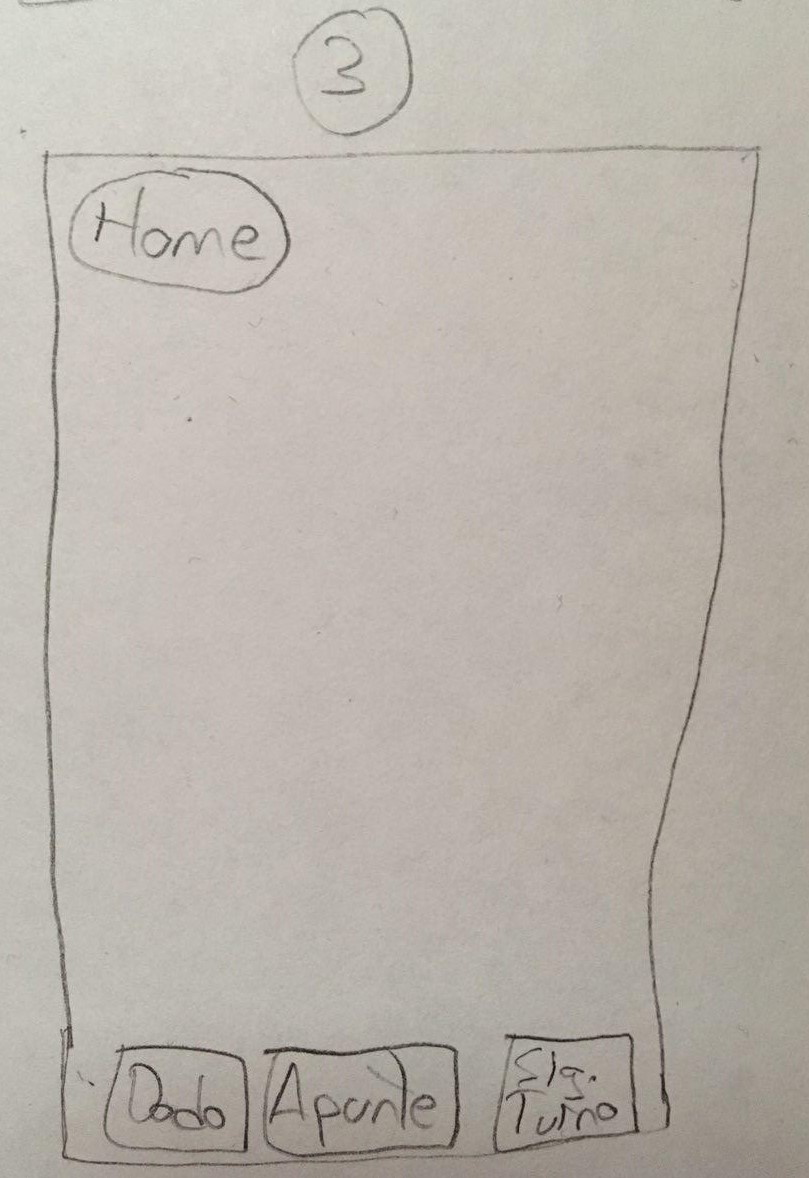
\includegraphics[height=2.47in]{b3.jpg}}
  \qquad
  \subfigure{
  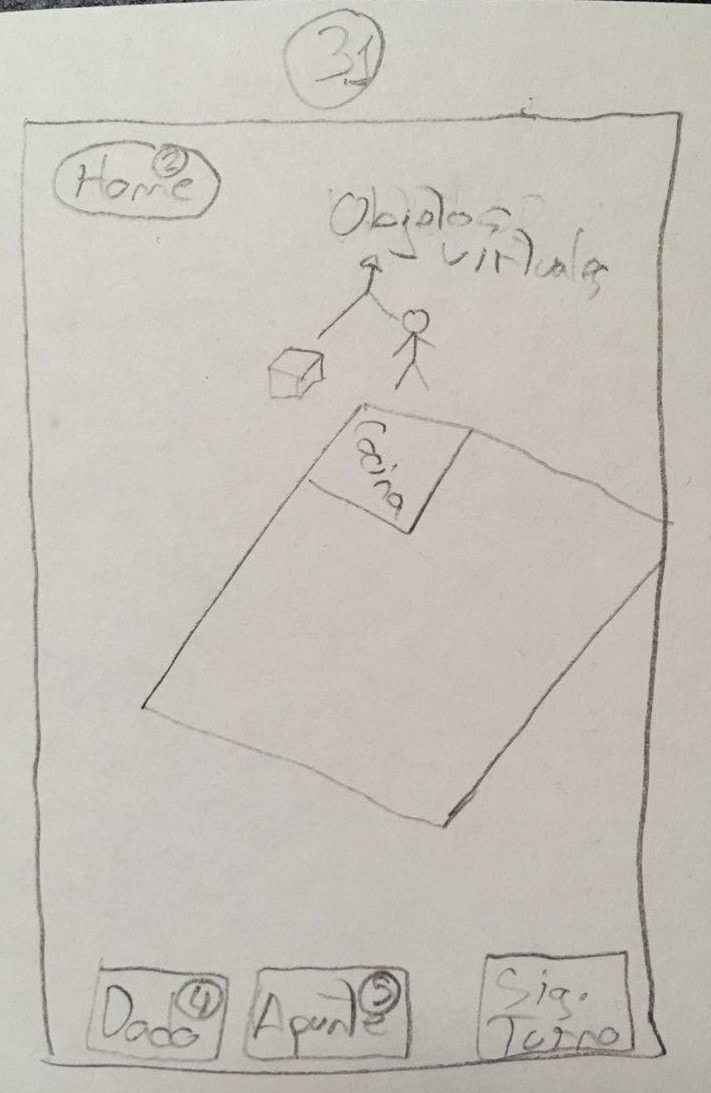
\includegraphics[height=2.52in]{b3-1.jpg}}
  \caption{Imagen que muestra los bocetos correspondientes a la interfaz de juego, en la derecha se esta escaneando el tablero.}
\end{figure}

\begin{figure}[h]
  \centering
  \subfigure{
  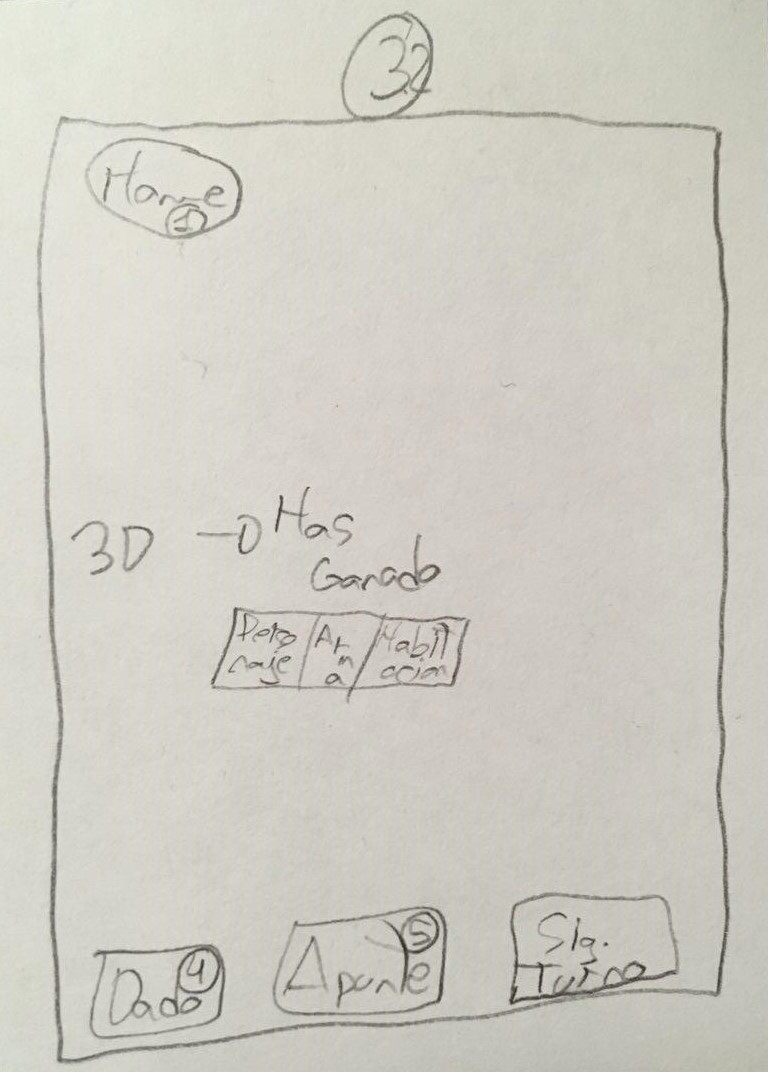
\includegraphics[height=2.5in]{b3-2.jpg}}
  \qquad
  \subfigure{
  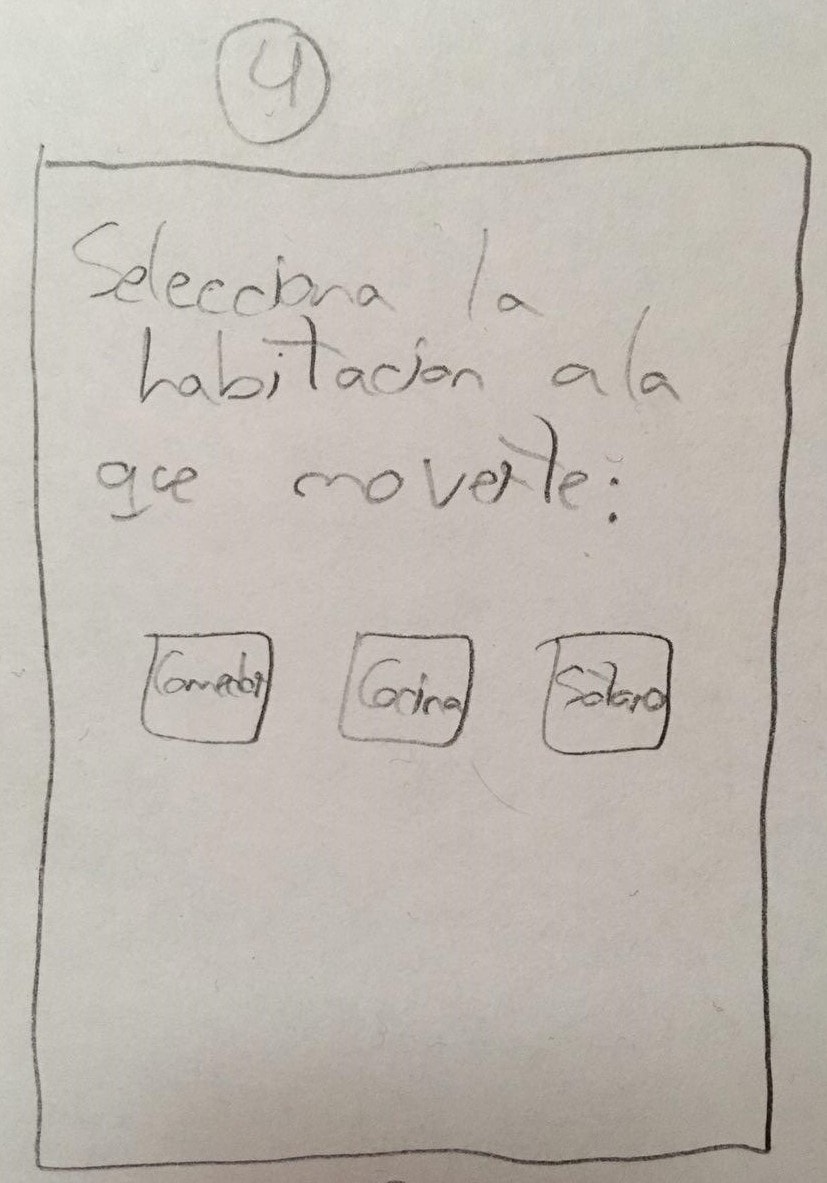
\includegraphics[height=2.5in]{b4.jpg}}
  \caption{Imagen que muestra los bocetos correspondientes a la interfaz de juego cuando se escanea una acusación, y a la interfaz de la seleción de habitación a la que moverse.}
\end{figure}

\begin{figure}[h]
  \centering
  \subfigure{
  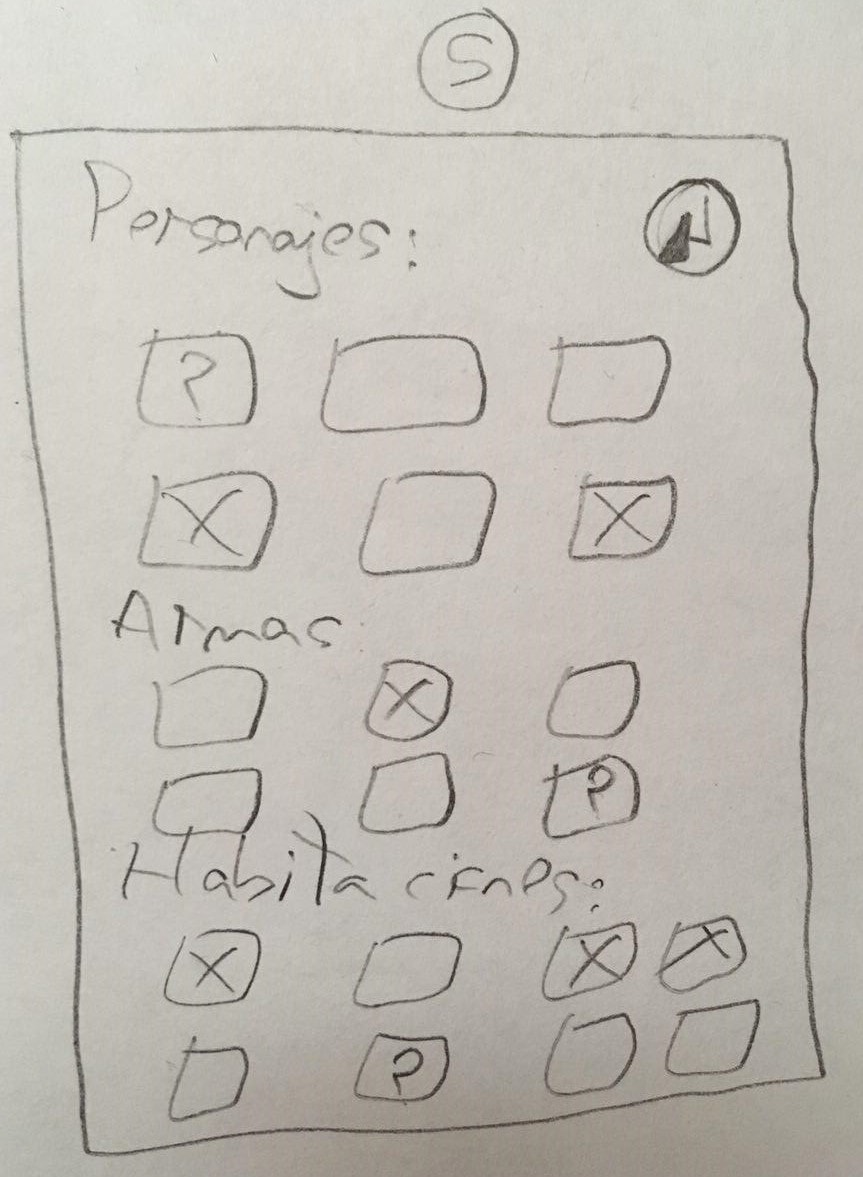
\includegraphics[height=2.5in]{b5.jpg}}
  \qquad
  \subfigure{
  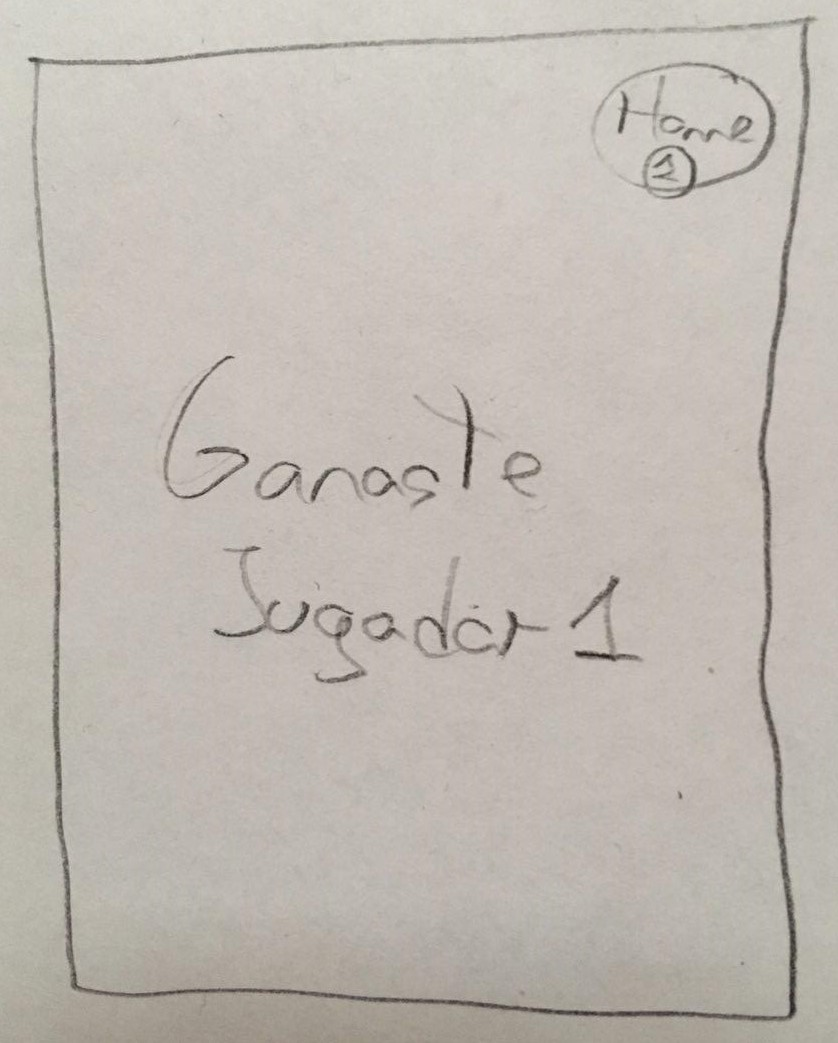
\includegraphics[height=2.5in]{b6.jpg}}
  \caption{Imagen que muestra los bocetos correspondientes a la interfaz de la toma de apuntes y la que indica que se ha ganado el juego.}
\end{figure}

\FloatBarrier

%%%%%%%%%%%%%%%%%%%%%%%%%%%%%%%%%%%%%%%%%%%%%%%%%%%%%% TABLAS USABILIDAD %%%%%%%%%%%%%%%%%%%%%%%%%%%%%%%%%%%%%%%%%%%%%%%%%%%%%%

\section{Tablas de usabilidad para los bocetos} \label{tablas-usabilidad-bocetos}

\begin{table}[!h]
  \begin{center}
    \begin{tabular}{|p{2.2cm}|p{1.9cm}|p{1.4cm}|p{1.2cm}|p{3.1cm}|p{3.1cm}|}

      \hline
        \rowcolor{Gray} \textbf{Escenario de uso}
        & \textbf{Tarea}
        & \textbf{Éxito/ Fracaso}
        & \textbf{Tiempo}
        & \textbf{Dificultades encontradas}
        & \textbf{Comentarios}\\

      \hline
      El usuario está jugando una partida
      & Seleccionar ajustes iniciales
      & Éxito
      & 10 seg
      & Le cuesta seleccionar el personaje con el dedo
      & Hacer los botones de personaje mas grandes\\

      \hline
      El usuario está jugando una partida
      & Comenzar el juego
      & Éxito
      & 5 seg
      & Ninguna
      &\\

      \hline
      El usuario está jugando una partida
      & Salir de las instrucciones
      & Éxito
      & 5 seg
      & Ninguna
      &\\

      \hline
      El usuario está jugando una partida
      & Escanear el tablero
      & Éxito
      & 10 seg
      & Ninguna
      &\\

      \hline
      El usuario está jugando una partida
      & Lanzar el dado
      & Éxito
      & 20 seg
      & Ninguna
      & Añadir imagen con el nombre de la habitación\\

      \hline
      El usuario está jugando una partida
      & Hacer apunte
      & Éxito
      & 25 seg
      & Ninguna
      &\\

      \hline
      El usuario está jugando una partida
      & Escanear acusación
      & Éxito
      & 20 seg
      & Ninguna
      &\\

      \hline
      El usuario está jugando una partida
      & Pasar de turno
      & Éxito
      & 5 seg
      & Ninguna
      &\\

      \hline
      El usuario está jugando una partida
      & Volver a la pantalla inicial
      & Fracaso
      & 15 seg
      & No sabe donde seleccionar terminar partida
      & Cambiar el texto del botón home por Terminar partida\\

      \hline
      El usuario está jugando una partida
      & Finalizar después de ganar
      & Éxito
      & 5 seg
      & No sabe donde seleccionar para salir de esa pantalla
      & Cambiar el texto del botón home por Continuar\\

      \hline

    \end{tabular}

    \caption{Resultados usabilidad con Usuario 1.}
    \label{tabla-bocetos-usuario1}

  \end{center}
\end{table}


\begin{table}[h]
  \begin{center}
    \begin{tabular}{|p{2.5cm}|p{1.75cm}|p{1.25cm}|p{1.25cm}|p{2.75cm}|p{3.5cm}|}

      \hline
        \rowcolor{Gray} \textbf{Escenario de uso}
        & \textbf{Tarea}
        & \textbf{Éxito/ Fracaso}
        & \textbf{Tiempo}
        & \textbf{Dificultades encontradas}
        & \textbf{Comentarios}\\

      \hline
      El usuario se encuentra jugando una partida
      & Seleccionar ajustes iniciales
      & Éxito
      & 5 seg
      & Ninguna
      &\\

      \hline
      El usuario se encuentra jugando una partida
      & Comenzar el juego
      & Éxito
      & 5 seg
      & Ninguna
      &\\

      \hline
      El usuario se encuentra jugando una partida
      & Salir de las instrucciones
      & Éxito
      & 5 seg
      & Ninguna
      &\\

      \hline
      El usuario se encuentra jugando una partida
      & Escanear el tablero
      & Éxito
      & 15 seg
      & Ninguna
      &\\

      \hline
      El usuario se encuentra jugando una partida
      & Lanzar el dado
      & Éxito
      & 10 seg
      & Ninguna
      & \\

      \hline
      El usuario se encuentra jugando una partida
      & Hacer apunte
      & Fracaso
      & 25 seg
      & No comprendía el funcionamiento de cómo realizar un apunte
      & Explicar en la pantalla de instrucciones inicial como se realiza un apunte\\

      \hline
      El usuario se encuentra jugando una partida
      & Escanear acusación
      & Éxito
      & 10 seg
      & Ninguna
      &\\

      \hline
      El usuario se encuentra jugando una partida
      & Pasar de turno
      & Éxito
      & 3 seg
      & Ninguna
      &\\

      \hline
      El usuario se encuentra jugando una partida
      & Volver a la pantalla inicial
      & Fracaso
      & 7 seg
      & No encontraba el botón de inicio
      & Cambiar el texto del botón a español y mas grande\\

      \hline
      El usuario se encuentra jugando una partida
      & Finalizar después de ganar
      & Éxito
      & 3 seg
      & No sabe que significa home, el botón es pequeño y poco accesible
      & Cambiar el texto del botón a español y mas grande\\

      \hline

    \end{tabular}

    \caption{Resultados usabilidad con Usuario 2.}
    \label{tabla-bocetos-usuario2}

  \end{center}
\end{table}


\begin{table}[h]
  \begin{center}
    \begin{tabular}{|p{2.5cm}|p{1.75cm}|p{1.25cm}|p{1.25cm}|p{2.75cm}|p{3.5cm}|}

      \hline
        \rowcolor{Gray} \textbf{Escenario de uso}
        & \textbf{Tarea}
        & \textbf{Éxito/ Fracaso}
        & \textbf{Tiempo}
        & \textbf{Dificultades encontradas}
        & \textbf{Comentarios}\\

      \hline
      El usuario se encuentra jugando una partida
      & Seleccionar ajustes iniciales
      & Éxito
      & 5 seg
      & Ninguna
      & Activar el botón de play cuando haya seleccionado 2 personajes\\

      \hline
      El usuario se encuentra jugando una partida
      & Comenzar el juego
      & Éxito
      & 5 seg
      & Ninguna
      &\\

      \hline
      El usuario se encuentra jugando una partida
      & Salir de las instrucciones
      & Éxito
      & 5 seg
      & Ninguna
      &\\

      \hline
      El usuario se encuentra jugando una partida
      & Escanear el tablero
      & Éxito
      & 3 seg
      & Ninguna
      &\\

      \hline
      El usuario se encuentra jugando una partida
      & Lanzar el dado
      & Éxito
      & 15 seg
      & El botón de dado no era muy descriptivo y el usuario no sabia si ahí se lanzaba
      & Cambiar el texto del botón dado a Lanzar dado\\

      \hline
      El usuario se encuentra jugando una partida
      & Hacer apunte
      & Éxito
      & 20 seg
      & El botón usuario no entiende que pasa al pulsar el botón de apunte
      & Cambiar el texto del botón de apunte a Notas\\

      \hline
      El usuario se encuentra jugando una partida
      & Escanear acusación
      & Éxito
      & 10 seg
      & Ninguna
      &\\

      \hline
      El usuario se encuentra jugando una partida
      & Pasar de turno
      & Éxito
      & 3 seg
      & Ninguna
      &\\

      \hline
      El usuario se encuentra jugando una partida
      & Volver a la pantalla inicial
      & Éxito
      & 3 seg
      & Ninguna
      &\\

      \hline
      El usuario se encuentra jugando una partida
      & Finalizar después de ganar
      & Éxito
      & 3 seg
      & Ninguna
      & Camiar el texto a Continuar y cambiar su posición y tamaño\\

      \hline

    \end{tabular}

    \caption{Resultados usabilidad con Usuario 3.}
    \label{tabla-bocetos-usuario3}

  \end{center}
\end{table}

\FloatBarrier

%%%%%%%%%%%%%%%%%%%%%%%%%%%%%%%%%%%%%%%%%%%%%%%%%%%%%% TABLAS USABILIDAD 2 %%%%%%%%%%%%%%%%%%%%%%%%%%%%%%%%%%%%%%%%%%%%%%%%%%%%%%

\section{Tablas de usabilidad para la Entrega 2} \label{tablas-usabilidad-entrega-2}

\begin{table}[h]
  \begin{center}
    \begin{tabular}{|p{2.5cm}|p{1.75cm}|p{1.25cm}|p{1.25cm}|p{2.75cm}|p{3.5cm}|}

      \hline
        \rowcolor{Gray} \textbf{Escenario de uso}
        & \textbf{Tarea}
        & \textbf{Éxito/ Fracaso}
        & \textbf{Tiempo}
        & \textbf{Dificultades encontradas}
        & \textbf{Comentarios}\\

      \hline
      El usuario se encuentra jugando una partida
      & Seleccionar ajustes iniciales
      & Éxito
      & 7 seg
      & Ninguna
      &\\

      \hline
      El usuario se encuentra jugando una partida
      & Comenzar el juego
      & Éxito
      & 1 seg
      & Ninguna
      &\\

      \hline
      El usuario se encuentra jugando una partida
      & Salir de las instrucciones
      & Éxito
      & 4 seg
      & Ninguna
      &\\

      \hline
      El usuario se encuentra jugando una partida
      & Escanear el tablero
      & Éxito
      & 12 seg
      & Ninguna
      &\\

      \hline

    \end{tabular}

    \caption{Resultados usabilidad en la Entrega 2 con Usuario 1.}
    \label{tabla-entrega-2-usuario1}

  \end{center}
\end{table}


\begin{table}[h]
  \begin{center}
    \begin{tabular}{|p{2.5cm}|p{1.75cm}|p{1.25cm}|p{1.25cm}|p{2.75cm}|p{3.5cm}|}

      \hline
        \rowcolor{Gray} \textbf{Escenario de uso}
        & \textbf{Tarea}
        & \textbf{Éxito/ Fracaso}
        & \textbf{Tiempo}
        & \textbf{Dificultades encontradas}
        & \textbf{Comentarios}\\

      \hline
      El usuario se encuentra jugando una partida
      & Seleccionar ajustes iniciales
      & Éxito
      & 5 seg
      & Ninguna
      &\\

      \hline
      El usuario se encuentra jugando una partida
      & Comenzar el juego
      & Éxito
      & 5 seg
      & Ninguna
      &\\

      \hline
      El usuario se encuentra jugando una partida
      & Salir de las instrucciones
      & Éxito
      & 5 seg
      & Ninguna
      &\\

      \hline
      El usuario se encuentra jugando una partida
      & Escanear el tablero
      & Éxito
      & 15 seg
      & Ninguna
      &\\

      \hline

    \end{tabular}

    \caption{Resultados usabilidad en la Entrega 2 con Usuario 2.}
    \label{tabla-entrega-2-usuario2}

  \end{center}
\end{table}


\begin{table}[h]
  \begin{center}
    \begin{tabular}{|p{2.5cm}|p{1.75cm}|p{1.25cm}|p{1.25cm}|p{2.75cm}|p{3.5cm}|}

      \hline
        \rowcolor{Gray} \textbf{Escenario de uso}
        & \textbf{Tarea}
        & \textbf{Éxito/ Fracaso}
        & \textbf{Tiempo}
        & \textbf{Dificultades encontradas}
        & \textbf{Comentarios}\\

      \hline
      El usuario se encuentra jugando una partida
      & Seleccionar ajustes iniciales
      & Éxito
      & 7 seg
      & Ninguna
      &\\

      \hline
      El usuario se encuentra jugando una partida
      & Comenzar el juego
      & Éxito
      & 1 seg
      & Ninguna
      &\\

      \hline
      El usuario se encuentra jugando una partida
      & Salir de las instrucciones
      & Éxito
      & 2 seg
      & Ninguna
      & Le cuesta leer el texto por la similitud de color con el fondo\\

      \hline
      El usuario se encuentra jugando una partida
      & Escanear el tablero
      & Éxito
      & 6 seg
      & Ninguna
      &\\

      \hline

    \end{tabular}

    \caption{Resultados usabilidad en la Entrega 2 con Usuario 3.}
    \label{tabla-entrega-2-usuario3}

  \end{center}
\end{table}

\FloatBarrier

%%%%%%%%%%%%%%%%%%%%%%%%%%%%%%%%%%%%%%%%%%%%%%%%%%%%%% TABLAS USABILIDAD 3 %%%%%%%%%%%%%%%%%%%%%%%%%%%%%%%%%%%%%%%%%%%%%%%%%%%%%%

\section{Tablas de usabilidad para la Entrega 3} \label{tablas-usabilidad-entrega-3}

\begin{table}[h]
  \begin{center}
    \begin{tabular}{|p{2.5cm}|p{1.75cm}|p{1.25cm}|p{1.25cm}|p{2.75cm}|p{3.5cm}|}

      \hline
        \rowcolor{Gray} \textbf{Escenario de uso}
        & \textbf{Tarea}
        & \textbf{Éxito/ Fracaso}
        & \textbf{Tiempo}
        & \textbf{Dificultades encontradas}
        & \textbf{Comentarios}\\

      \hline
      El usuario se encuentra jugando una partida
      & Lanzar el dado
      & Éxito
      & 9 seg
      & Ninguna
      & Añadir indicador al personaje actual para saber su posicion en todo momento\\

      \hline
      El usuario se encuentra jugando una partida
      & Hacer apunte
      & Éxito
      & 16 seg
      & Ninguna
      &\\

      \hline
      El usuario se encuentra jugando una partida
      & Escanear acusación
      & Éxito
      & 20 seg
      & Le cuesta escanear las cartas, ya que el juego tarda en detectarla
      &\\

      \hline
      El usuario se encuentra jugando una partida
      & Volver a la pantalla inicial
      & Éxtio
      & 3 seg
      & Ninguna
      &\\

      \hline
      El usuario se encuentra jugando una partida
      & Finalizar después de ganar
      & Éxito
      & 1 seg
      & Ninguna
      &\\

      \hline

    \end{tabular}

    \caption{Resultados usabilidad en la Entrega 3 con Usuario 1.}
    \label{tabla-entrega-3-usuario1}

  \end{center}
\end{table}


\begin{table}[h]
  \begin{center}
    \begin{tabular}{|p{2.5cm}|p{1.75cm}|p{1.25cm}|p{1.25cm}|p{2.75cm}|p{3.5cm}|}

      \hline
        \rowcolor{Gray} \textbf{Escenario de uso}
        & \textbf{Tarea}
        & \textbf{Éxito/ Fracaso}
        & \textbf{Tiempo}
        & \textbf{Dificultades encontradas}
        & \textbf{Comentarios}\\

      \hline
      El usuario se encuentra jugando una partida
      & Lanzar el dado
      & Éxito
      & 10 seg
      & Ninguna
      & \\

      \hline
      El usuario se encuentra jugando una partida
      & Hacer apunte
      & Fracaso
      & 25 seg
      & No comprendía el funcionamiento de cómo realizar un apunte
      & Explicar en la pantalla de instrucciones inicial como se realiza un apunte\\

      \hline
      El usuario se encuentra jugando una partida
      & Escanear acusación
      & Éxito
      & 10 seg
      & Ninguna
      &\\

      \hline
      El usuario se encuentra jugando una partida
      & Volver a la pantalla inicial
      & Fracaso
      & 7 seg
      & No encontraba el botón de inicio
      & Cambiar el texto del botón a español y mas grande\\

      \hline
      El usuario se encuentra jugando una partida
      & Finalizar después de ganar
      & Éxito
      & 3 seg
      & No sabe que significa home, el botón es pequeño y poco accesible
      & Cambiar el texto del botón a español y mas grande\\

      \hline

    \end{tabular}

    \caption{Resultados usabilidad en la Entrega 3 con Usuario 2.}
    \label{tabla-entrega-3-usuario2}

  \end{center}
\end{table}


\begin{table}[h]
  \begin{center}
    \begin{tabular}{|p{2.5cm}|p{1.75cm}|p{1.25cm}|p{1.25cm}|p{2.75cm}|p{3.5cm}|}

      \hline
        \rowcolor{Gray} \textbf{Escenario de uso}
        & \textbf{Tarea}
        & \textbf{Éxito/ Fracaso}
        & \textbf{Tiempo}
        & \textbf{Dificultades encontradas}
        & \textbf{Comentarios}\\

      \hline
      El usuario se encuentra jugando una partida
      & Lanzar el dado
      & Éxito
      & 4 seg
      & Le cuesta leer los cubos(botones)
      &\\

      \hline
      El usuario se encuentra jugando una partida
      & Hacer apunte
      & Éxito
      & 10 seg
      & Ninguna
      &\\

      \hline
      El usuario se encuentra jugando una partida
      & Escanear acusación
      & Éxito
      & 20 seg
      & Ninguna
      &\\

      \hline
      El usuario se encuentra jugando una partida
      & Volver a la pantalla inicial
      & Éxito
      & 6 seg
      & Ninguna
      &\\

      \hline
      El usuario se encuentra jugando una partida
      & Finalizar después de ganar
      & Éxito
      & 3 seg
      & Ninguna
      &\\

      \hline

    \end{tabular}

    \caption{Resultados usabilidad en la Entrega 3 con Usuario 3.}
    \label{tabla-entrega-3-usuario3}

  \end{center}
\end{table}

\FloatBarrier

%%%%%%%%%%%%%%%%%%%%%%%%%%%%%%%%%%%%%%%%%%%%%%%%%%%%%% TABLAS USABILIDAD 4 %%%%%%%%%%%%%%%%%%%%%%%%%%%%%%%%%%%%%%%%%%%%%%%%%%%%%%

\section{Tablas de usabilidad para la Entrega 4} \label{tablas-usabilidad-entrega-4}

\begin{table}[h]
  \begin{center}
    \begin{tabular}{|p{2.5cm}|p{1.75cm}|p{1.25cm}|p{1.25cm}|p{2.75cm}|p{3.5cm}|}

      \hline
        \rowcolor{Gray} \textbf{Escenario de uso}
        & \textbf{Tarea}
        & \textbf{Éxito/ Fracaso}
        & \textbf{Tiempo}
        & \textbf{Dificultades encontradas}
        & \textbf{Comentarios}\\

        \hline
        El usuario se encuentra jugando una partida
        & Pasar de turno
        & Éxito
        & 2 seg
        & Ninguna
        &\\

      \hline

    \end{tabular}

    \caption{Resultados usabilidad en la Entrega 4 con Usuario 1.}
    \label{tabla-entrega-4-usuario1}

  \end{center}
\end{table}


\begin{table}[h]
  \begin{center}
    \begin{tabular}{|p{2.5cm}|p{1.75cm}|p{1.25cm}|p{1.25cm}|p{2.75cm}|p{3.5cm}|}

      \hline
        \rowcolor{Gray} \textbf{Escenario de uso}
        & \textbf{Tarea}
        & \textbf{Éxito/ Fracaso}
        & \textbf{Tiempo}
        & \textbf{Dificultades encontradas}
        & \textbf{Comentarios}\\

        \hline
        El usuario se encuentra jugando una partida
        & Pasar de turno
        & Éxito
        & 5 seg
        & Ninguna
        &\\

      \hline

    \end{tabular}

    \caption{Resultados usabilidad en la Entrega 4 con Usuario 2.}
    \label{tabla-entrega-4-usuario2}

  \end{center}
\end{table}


\begin{table}[h]
  \begin{center}
    \begin{tabular}{|p{2.5cm}|p{1.75cm}|p{1.25cm}|p{1.25cm}|p{2.75cm}|p{3.5cm}|}

      \hline
        \rowcolor{Gray} \textbf{Escenario de uso}
        & \textbf{Tarea}
        & \textbf{Éxito/ Fracaso}
        & \textbf{Tiempo}
        & \textbf{Dificultades encontradas}
        & \textbf{Comentarios}\\

        \hline
        El usuario se encuentra jugando una partida
        & Pasar de turno
        & Éxito
        & 2 seg
        & Ninguna
        &\\

      \hline

    \end{tabular}

    \caption{Resultados usabilidad en la Entrega 4 con Usuario 3.}
    \label{tabla-entrega-4-usuario3}

  \end{center}
\end{table}
